\documentclass[a4paper,11pt,fleqn]{scrartcl}%fleqn pour aligner les equations à gauche
\usepackage{../../Styles/Cours}


\newcommand{\chnum}{Chapitre 13}
\newcommand{\chtitle}{Variation du vecteur vitesse en chute libre}
\newcommand{\dtype}{TP}

\begin{document}
	\maketitle
    On étudie le movement d'un gymnaste lors d'un saut vertical au trampoline. Son saut atteint une hauteur maximale de \SI{8}{m}. Il reste alors environ \SI{2}{s} en l'air pour effectuer sa figure.\\

    \noindent\begin{minipage}{.5\linewidth}
    \begin{documentboxenv}{Saut en trampoline}
        En trampoline, les gymnastes évoluent sur une toile de \SI{4}{m} sur 2 située à \SI{1,15}{m} du sol.
        \begin{center}
            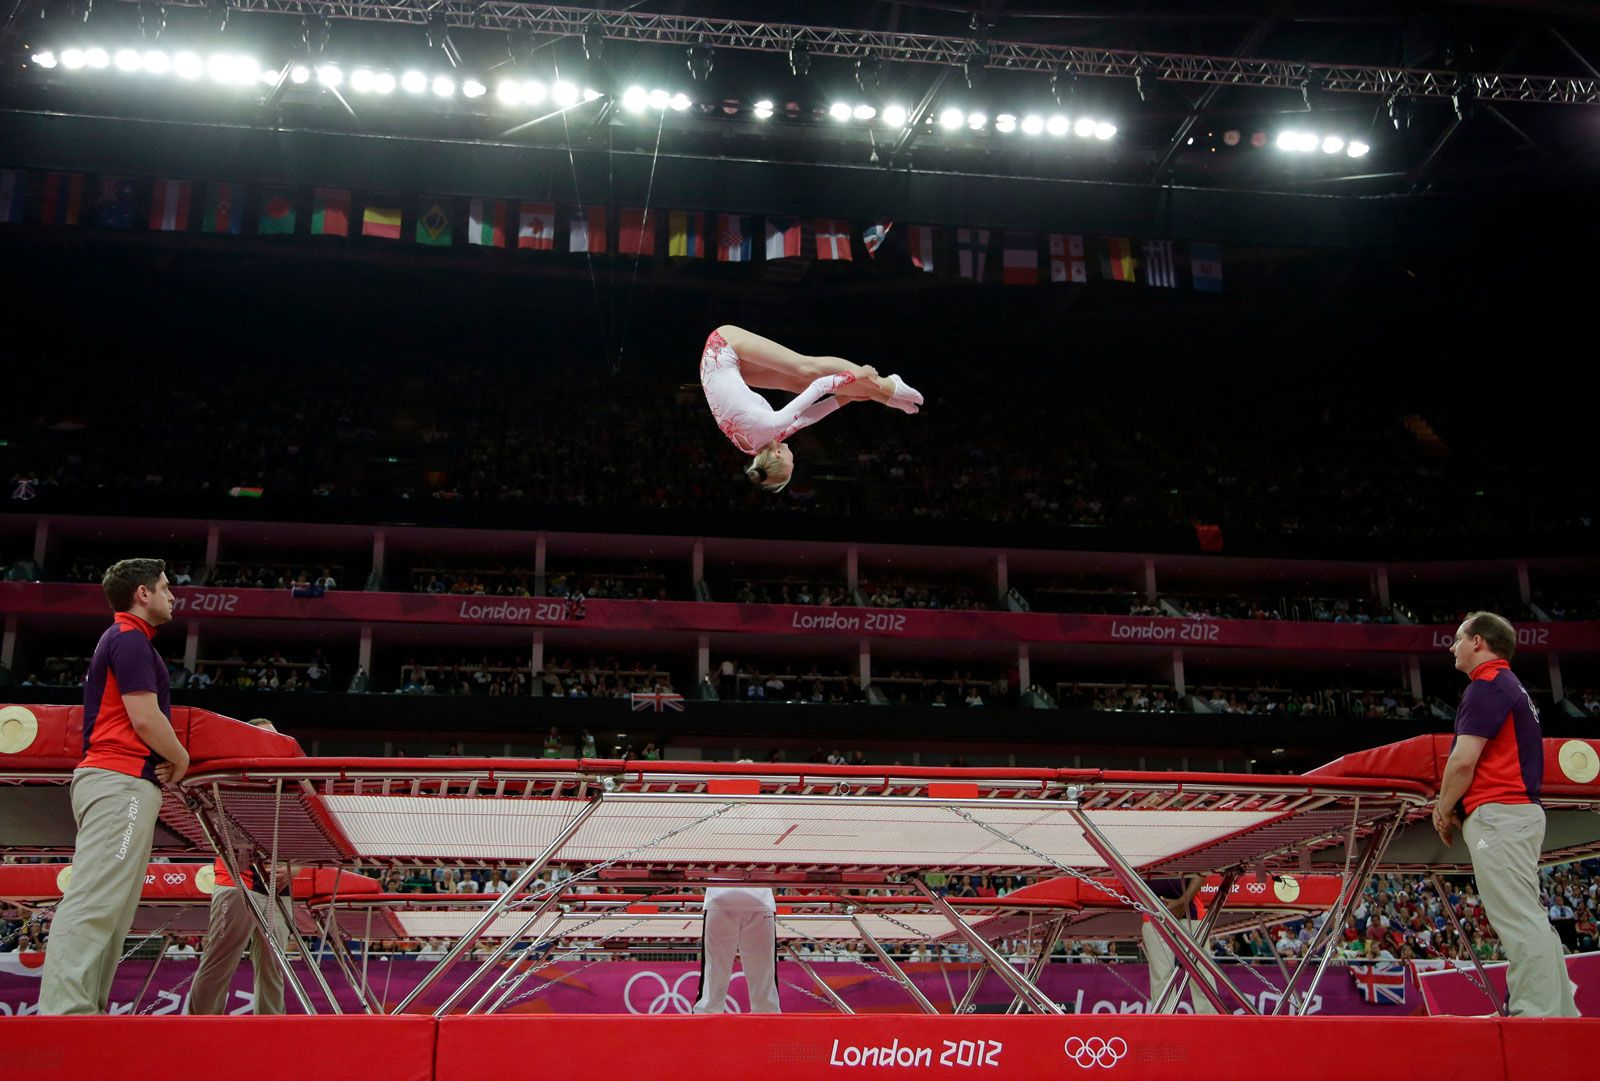
\includegraphics[width=\linewidth]{Ressources/trampoline.jpg}
        \end{center}
    \end{documentboxenv}
    \end{minipage}
    \begin{minipage}{.49\linewidth}
        \begin{documentboxenv}{Chronophotographie du centre de gravité du gymnaste}
        \begin{center}
            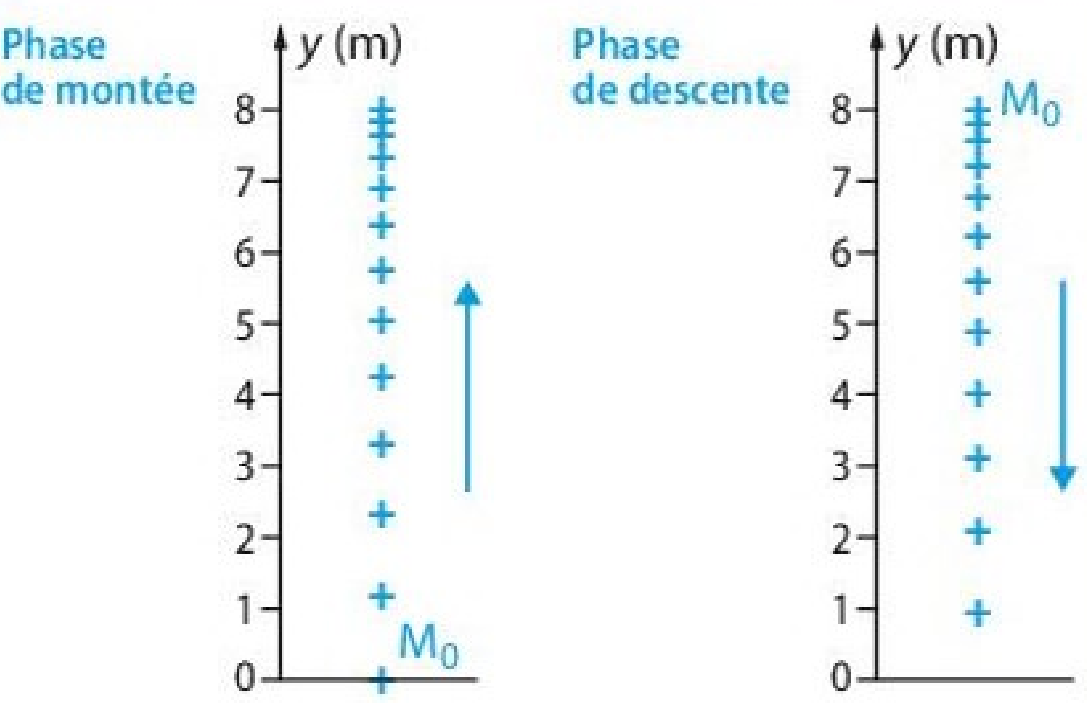
\includegraphics[width=.92\linewidth]{Ressources/Gymnaste_Chronophoto.png}
        \end{center}
        Entre deux positions successives du gymnaste il s'écoule une durée égale à \SI{100}{\milli\second}.
        \end{documentboxenv}
    \end{minipage}

    \noindent\begin{minipage}{\linewidth}
        \begin{documentboxenv}{Vitesses du centre de gravité du gymnaste}
        \label{doc3}
            Lors de la montée
            \begin{center}
                \begin{tabular}{|c|c|c|c|c|c|c|c|c|c|c|c|c|c|}
                    \hline
                    $t(\unit{\second})$ & 0.00&0.10&0.20&0.30&0.40&0.50&0.60&0.70&0.80&0.90&1.0&1.1&1.2\\
                    \hline
                    $v(\unit{\meter\per\second})$&12.5&11.6&10.6&9.61&8.63&7.65&6.67&5.69&4.71&3.73&2.75&1.77&0.79\\
                    \hline
                \end{tabular}
            \end{center}
            Lors de la descente
            \begin{center}
                \begin{tabular}{|c|c|c|c|c|c|c|c|c|c|c|c|c|c|}
                    \hline
                    $t$ (\unit{\second}) & 0.00&0.10&0.20&0.30&0.40&0.50&0.60&0.70&0.80&0.90&1.0&1.1&1.2\\
                    \hline
                    $v$ (\unit{\meter\per\second})&0.0&1.00&2.00&2.94&3.92&4.90&5.88&6.86&7.84&8.82&9.80&10.8&11.8\\
                    \hline
                \end{tabular}
            \end{center}
        \end{documentboxenv}
    \end{minipage}
    \begin{question}
        \begin{enumerate}
            \item Sans soucis d'échelle, représenter sur un schéma la force qui s'exerce sur le gymnaste en vol dans les deux phases du mouvement en indiquant le référentel d'étude choisi. Les forces de frottement de l'air sont négligées.
            \item A l'aide du Doc.~\ref{doc3}, décrire comment évolue lavitesse du gymnaste dans les phases ascendante et descendante.
            \item Pour les deux phases, dessiner en rouge les vecteurs vitesse $\vv{v_1}$, $\vv{v_2}$,$\vv{v_8}$ et $\vv{v_9}$ avec une échelle judicieusement choisie.
            \item Pour les deux phases, calculer et tracer les vecteurs $\Delta \vv{v_2}$ et $\Delta \vv{v_9}$ sachant que  $\Delta \vv{v_2} = \vv{v_2} - \vv{v_1}$.
            \item Décrire la direction, le sens et la variation d'intensité du vecteur  $\Delta \vv{v}$ dans les deux phases du mouvement.
            \item Identifier la force responsable de la variation du vetceur vitesse.
        \end{enumerate}
    \end{question}
\end{document}